\chapter{The charts}

Charts are computed from the project's own numbers --- each plotted series is a fact from the
ladder contract, the budget proof or the measured benchmarks.

\section{The BPW grid (all 69 formats on the exact grid)}

\begin{center}
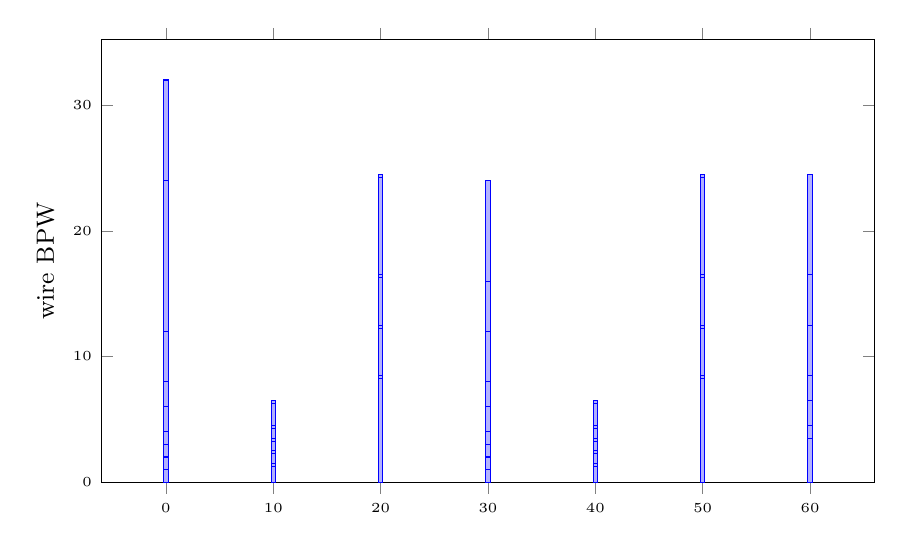
\begin{tikzpicture}
\begin{axis}[
  width=0.94\textwidth, height=7.2cm,
  ybar, bar width=1.6pt,
  ymin=0, ylabel={wire BPW},
  symbolic x coords={0,10,20,30,40,50,60},
  xtick=data,
  tick label style={font=\tiny},
  label style={font=\small},
  title style={font=\small},
]
\addplot coordinates {
  (0,1.00) (0,1.00) (0,2.00) (0,3.00) (0,4.00) (0,6.00) (0,8.00) (0,12.00) (0,24.00) (0,32.00)
  (10,1.25) (10,1.50) (10,2.25) (10,2.50) (10,3.25) (10,3.50) (10,4.25) (10,4.50) (10,6.25) (10,6.50)
  (20,8.25) (20,8.50) (20,12.25) (20,12.50) (20,16.25) (20,16.50) (20,24.25) (20,24.50)
  (30,1.00) (30,2.00) (30,3.00) (30,4.00) (30,6.00) (30,8.00) (30,12.00) (30,16.00) (30,24.00)
  (40,1.25) (40,1.50) (40,2.25) (40,2.50) (40,3.25) (40,3.50) (40,4.25) (40,4.50) (40,6.25) (40,6.50)
  (50,8.25) (50,8.50) (50,12.25) (50,12.50) (50,16.25) (50,16.50) (50,24.25) (50,24.50)
  (60,3.50) (60,4.50) (60,6.50) (60,8.50) (60,12.50) (60,16.50) (60,24.50)
};
\end{axis}
\end{tikzpicture}

\small Figure 1: the 69-format wire grid --- every bar lands on the $.0/.25/.50$ lattice; no
gaps, no 3.78125, no 2.625 (rule D-06).
\end{center}

\section{Memory: linear vs constant}

\begin{center}
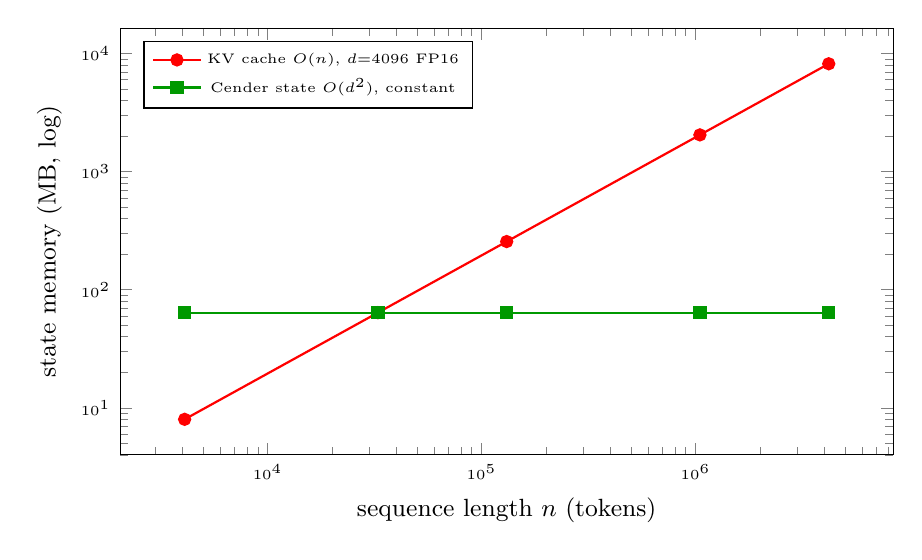
\begin{tikzpicture}
\begin{axis}[
  width=0.94\textwidth, height=7.0cm,
  xlabel={sequence length $n$ (tokens)}, ylabel={state memory (MB, log)},
  xmode=log, ymode=log, tick label style={font=\tiny},
  label style={font=\small},
  legend style={font=\tiny, at={(0.03,0.97)}, anchor=north west},
]
\addplot[color=red, thick, mark=*] coordinates {
  (4096,8) (32768,64) (131072,256) (1048576,2048) (4194304,8192)
};
\addlegendentry{KV cache $O(n)$, $d{=}4096$ FP16}
\addplot[color=green!60!black, thick, mark=square*] coordinates {
  (4096,64) (32768,64) (131072,64) (1048576,64) (4194304,64)
};
\addlegendentry{Cender state $O(d^2)$, constant}
\end{axis}
\end{tikzpicture}

\small Figure 2: Theorem~\ref{thm:memory} as a chart --- the KV cache grows linearly (8~MB at
4K $\to$ 8~GB at 4M); the Cender state stays at 64~MB. The ${\approx}1000\times$ ratio at
$n{=}4$M is visible as the vertical gap between the curves.
\end{center}

\section{Golden-section convergence (the scale fitter)}

\begin{center}
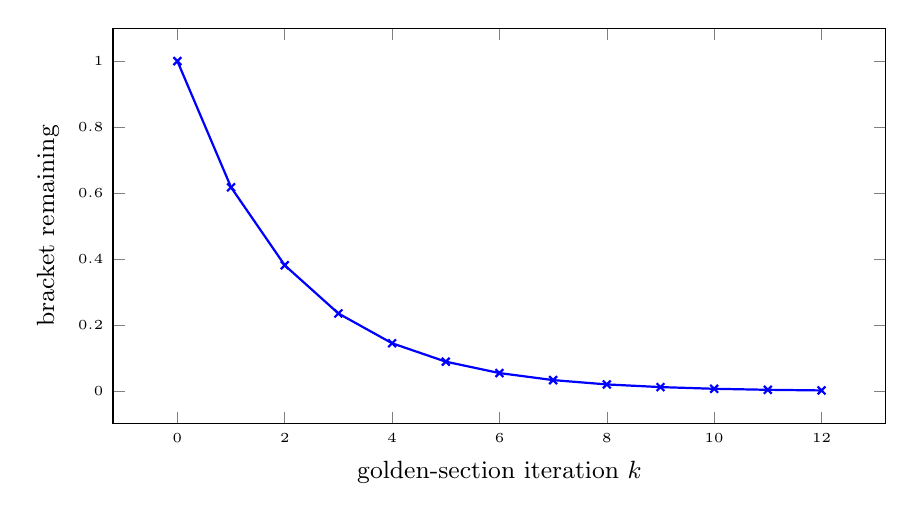
\begin{tikzpicture}
\begin{axis}[
  width=0.94\textwidth, height=6.6cm,
  xlabel={golden-section iteration $k$}, ylabel={bracket remaining},
  domain=0:12, samples=13,
  tick label style={font=\tiny},
  label style={font=\small},
]
\addplot[color=blue, thick, mark=x] coordinates {
  (0,1.0000) (1,0.6180) (2,0.3820) (3,0.2361) (4,0.1459) (5,0.0902)
  (6,0.0557) (7,0.0344) (8,0.0213) (9,0.0132) (10,0.0081) (11,0.0050) (12,0.0031)
};
\end{axis}
\end{tikzpicture}

\small Figure 3: the scale fitter's bracket shrinks by $\varphi \approx 0.618$ per iteration
($0.618^{12} \approx 0.0031$) --- twelve iterations resolve the scale to FP16 resolution
(D-12). The old 3-iteration LS seed measured 46~dB; 24 golden-section iterations reach
${\sim}59$~dB.
\end{center}

\section{The tier arithmetic}

\begin{center}
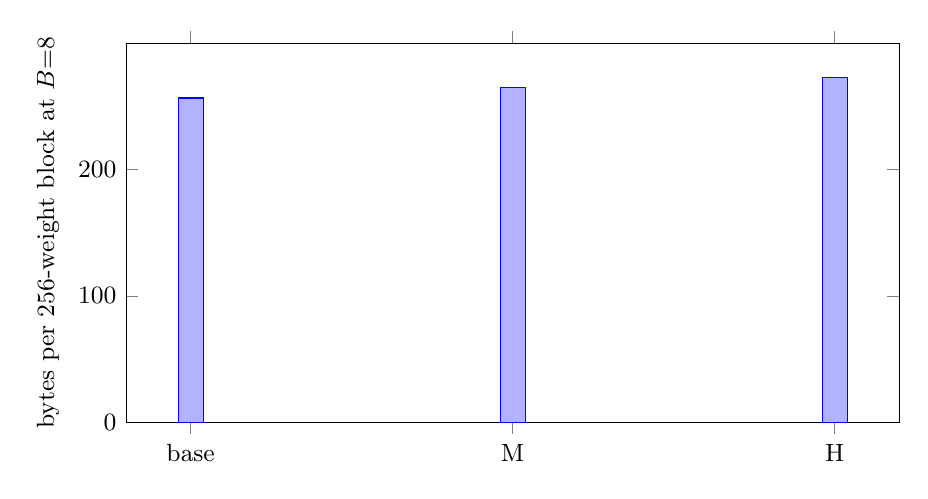
\begin{tikzpicture}
\begin{axis}[
  width=0.94\textwidth, height=6.4cm,
  ybar, bar width=9pt,
  symbolic x coords={base, M, H},
  ymin=0, ylabel={bytes per 256-weight block at $B{=}8$},
  xtick=data,
  tick label style={font=\small},
  label style={font=\small},
]
\addplot coordinates {(base,256) (M,264) (H,272)};
\end{axis}
\end{tikzpicture}

\small Figure 4: tier arithmetic at $B{=}8$ --- base 256 bytes, M $+8$ bytes (exactly
$+0.25$ BPW, D-09), H $+16$ bytes (exactly $+0.50$ BPW). The refinement bytes are the whole
tier difference; the quality gates order M strictly between L and H.
\end{center}

\section{The measured PTQ gap (looped models)}

\begin{center}
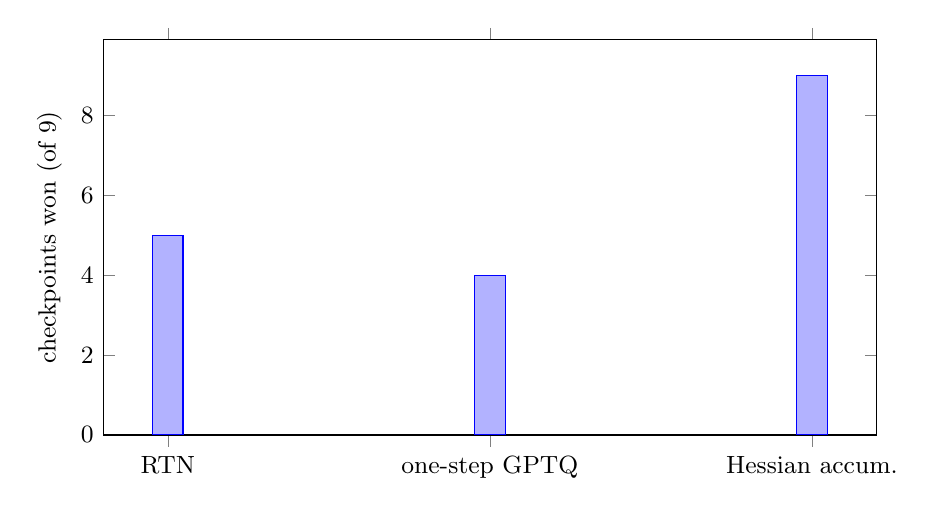
\begin{tikzpicture}
\begin{axis}[
  width=0.94\textwidth, height=6.6cm,
  ybar, bar width=11pt,
  symbolic x coords={RTN, one-step GPTQ, Hessian accum.},
  ymin=0, ylabel={checkpoints won (of 9)},
  xtick=data,
  tick label style={font=\small},
  label style={font=\small},
]
\addplot coordinates {(RTN,5) (one-step GPTQ,4) (Hessian accum.,9)};
\end{axis}
\end{tikzpicture}

\small Figure 5: the 2609.30820 result as a chart --- one-step GPTQ (calibration blindness)
loses to RTN on the primary metric for 5 of 9 looped checkpoints; Hessian accumulation across
recurrence steps wins 9/9 (Theorem~\ref{thm:hessian}).
\end{center}
